\section{REST-for-Physics libraries}

\label{sec:libraries}
% We define the different libraries in REST with a short description. We dedicate a section to the detector library since it is a central library that connects raw, geant4, and track libraries. And since REST was born to be used in the domain of rare event physics we always need a detector, but we are not forced to use it.

The main framework contains common tools required for centralized data access, visualization, and basic analysis routines, including generic \emph{REST-for-Physics} \emph{metadata} objects and \emph{processes} that do not require \emph{event} specialization, i.e. they only need to access information at the \emph{analysis tree} level. More specialized routines, requiring a dedicated \emph{event} data type, such as time signal processing or detector event reconstruction, are organized into libraries where all objects belonging to the library keep a closer relation and therefore enhanced connectivity. 

A library is usually associated only to one or two \emph{event} data types, improving the connectivity between different \emph{processes} inside the same library. This allows that processes "living" inside a particular library can be connected at any order and combination, as defined by the user. A dedicated library, the \emph{connectors} library, hosts those \emph{processes} or \emph{metadata} objects that need to interconnect different libraries, keeping all inter-library dependencies bounded together into a single entity, and allowing each library to be fully operational in stand-alone mode. New libraries might be added in the future to the framework, here we briefly describe those fundamental libraries that gave \emph{REST-for-Physics} enough functionality and versatility to be used in different aspects of rare event searches experiments.

\subsection{The detector library}

The detector library\footnote{\url{https://github.com/rest-for-physics/detectorlib}} is mainly used for event reconstruction inside a Time Projection Chamber (TPC). This library contains metadata objects that allow to describe the detector configuration and properties, such as the gas   in to define a detector readout topology, and access gas or other detector properties. It also implements processes including routines for event reconstruction from real detector data, and/or emulation of different physical response effects, such as electron diffusion.

\begin{figure}[hb!]
  \centering
  \raisebox{-0.5\height}{\includegraphics[width=0.3\linewidth]{images/stripped.pdf}\includegraphics[width=0.3\linewidth]{images/pixel.pdf}\includegraphics[width=0.3\linewidth]{images/microbulk.pdf}}
	\caption{}\label{fig:readouts}
\end{figure}

\subsection{The raw library}

The raw library\footnote{\url{https://github.com/rest-for-physics/rawlib}} is used to store time event pulses with a fixed number of bins. It includes processes related to signal conditioning, such as signal shaping, deconvolution, pulse fitting, de-noising, FFT, common noise reduction, and related routines. It is capable to read different binary formats from different electronic systems into REST.

\subsection{The geant4 library}
the geant4 library\footnote{\url{https://github.com/rest-for-physics/geant4lib}} is used to store and analyse the events generated in a Geant4 simulation, it defines and stores the particle generator and simulation conditions, such as the details of the physics list used during the Monte Carlo.

\subsection{The track library}

The track library\footnote{\url{https://github.com/rest-for-physics/tracklib}} defines a track event type allowing to define inheritance relations between tracks that contain groups of hits. A process connecting to the detector library allows for hit clustering to create a first set of tracks using a distance relation. Graph theory processes are included in this library in order to identify and reconstruct a physical track, and execute topological algorithms.

\subsection{The connectors library}

The connectors library\footnote{\url{https://github.com/rest-for-physics/connectorslib}} contains different processes that inter-connect fundamental REST libraries, requiring to transfer an event type into another. I.e. hit clustering to transform detector hits into a track event, or raw signal to be transformed into a detector event. It also may contain other complex processes that require to use 2 libraries simultaneously.

\begin{figure}[hb!]
  \centering
  \raisebox{-0.5\height}{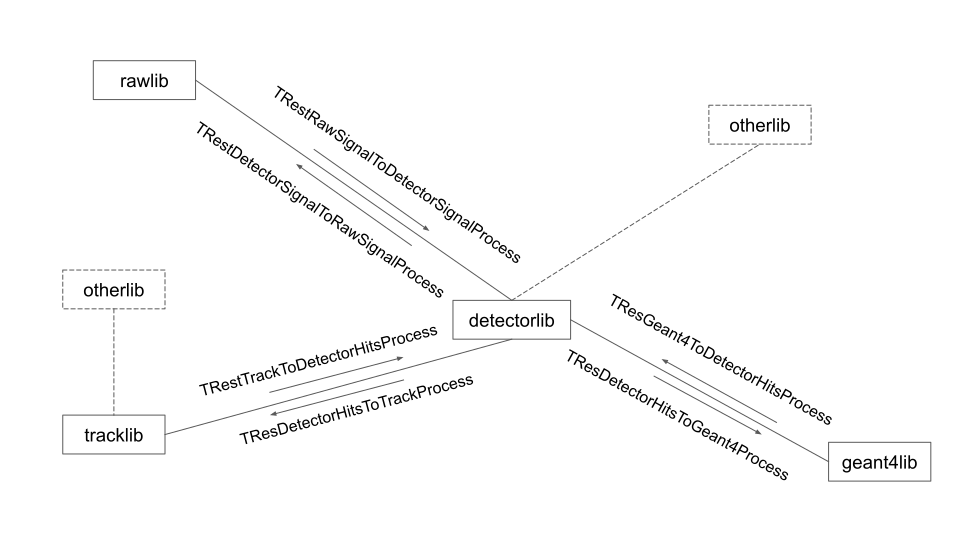
\includegraphics[width=0.75\linewidth]{images/connectorslib.png}}
	\caption{}\label{fig:connectorslib}
\end{figure}




